% !TEX root = ../../Tesi_Triennale_PMNS.tex
\chapter[cWB]{cWB: proprietà dell'algoritmo per la rivelazione e la ricostruzione di segnali di onde gravitazionali}
\label{chapter:cwb}

I metodi coerenti le statistiche vengono calcolate come somma coerente delle risposte dei detector singoli. Gli algoritmi che sfruttano questi metodi devono risultare più efficienti, devono cioè avere una probabilità di falso allarme più bassa, rispetto alle statistiche calcolate sulle risposte di ogni detector singolarmente.

L'algoritmo che si utilizza, Coherent WaveBurst (cWB), differisce dai metodi tradizionali che identificano gli eventi nei detector singolarmente usando statistiche di eccesso di potenza e poi verificano la coerenza tra i segnali nei vari detector. Esso utilizza infatti i dati di tutti i detector in un'unica statistica coerente costituita da una analisi della massima likelihood. 
I vantaggi di questo tipo di analisi sono molteplici: innanzitutto la sensibilità del metodo non sarà limitata dal detector meno sensibile nel network, in quanto la likelihood utilizzata nei metodi coerenti rappresenta il rapporto segnale su rumore (SNR) totale del segnale ricostruito/rivelato dal network. Inoltre questo metodo permette di costruire altre statistiche coerenti, come il null stream o il coefficiente di correlazione  del network, per distinguere segnali che effettivamente hanno una controparte fisica rispetto a eccessi di rumore ambientale o strumentale. Infine è possibile ricostruire la posizione celeste della sorgente.
\section{Analisi coerente}
La pipeline di cWB per rivelare e ricostruire segnali utilizza un metodo basato sul funzionale rapporto di verosimiglianza, che, in un'ipotesi idealistica di rumore gaussiano quasi stazionario, può essere scritto nel dominio di wavelet (in un piano tempo-frequenza) come
\begin{equation}
	\mathcal{L} = \sum_{k=1}^{K}\sum_{i,j=1}^{N}\left(\frac{w_k^2[i,j]}{\sigma_k^2[i,j]} - \frac{(w_k[i,j]-\xi_k[i,j])^2}{\sigma_k^2[i,j]}  \right)
\end{equation}
dove K è il numero di detector nel network, $w_k[i,j]$ è il campione di dati del detector (l'indice i itera sui tempi, mentre l'indice j itera sulle frequenze) e infine $\xi_k[i,j]$ è la risposta del detector k-esimo.
Il rumore del detector è è caratterizzato dalla deviazione standard $\sigma_k[i,j]$ che può variare lungo il piano tempo-frequenza.
Le risposte del network sono scritte come
\begin{equation}
	\xi_k[i,j] = F_{+,k}h_+[i,j] + F_{\times,k}h_\times[i,j]
\end{equation}
dove $F_{+,k}(\theta,\phi)$ e $F_{\times,k}(\theta,\phi)$ sono gli antenna pattern del detector k-esimo

Antenna pattern. The radiation pattern or antenna pattern is the graphical representation of the radiation properties of the antenna as a function of space. That is, the antenna's pattern describes how the antenna radiates energy out into space (or how it receives energy). It is important to state that an antenna radiates energy in all directions, at least to some extent, so the antenna pattern is actually three-dimensional. It is common, however, to describe this 3D pattern with two planar patterns, called the principal plane patterns. These principal plane patterns can be obtained by making two slices through the 3D pattern through the maximum value of the pattern or by direct measurement. It is these principal plane patterns that are commonly referred to as the antenna patterns. 

Introduzione sull'algoritmo fatta nel paragrafo precedente, magari riprenderla velocemente.

Coherent analysis, significato e descrizione della likelihood: spiega quindi bene la differenza con gli algoritmi classici di confronto con segnali già modellati.

regolatori, antenna pattern

algoritmi utilizzati: wavelet transformation, (linear predicion error), mappa verosimiglianza, mappa energia coerente (con piccoli grafici esemplificativi)

(cenni sulla trasformazione di fase)

\begin{center}
	\begin{figure}[ht]
		\centering
		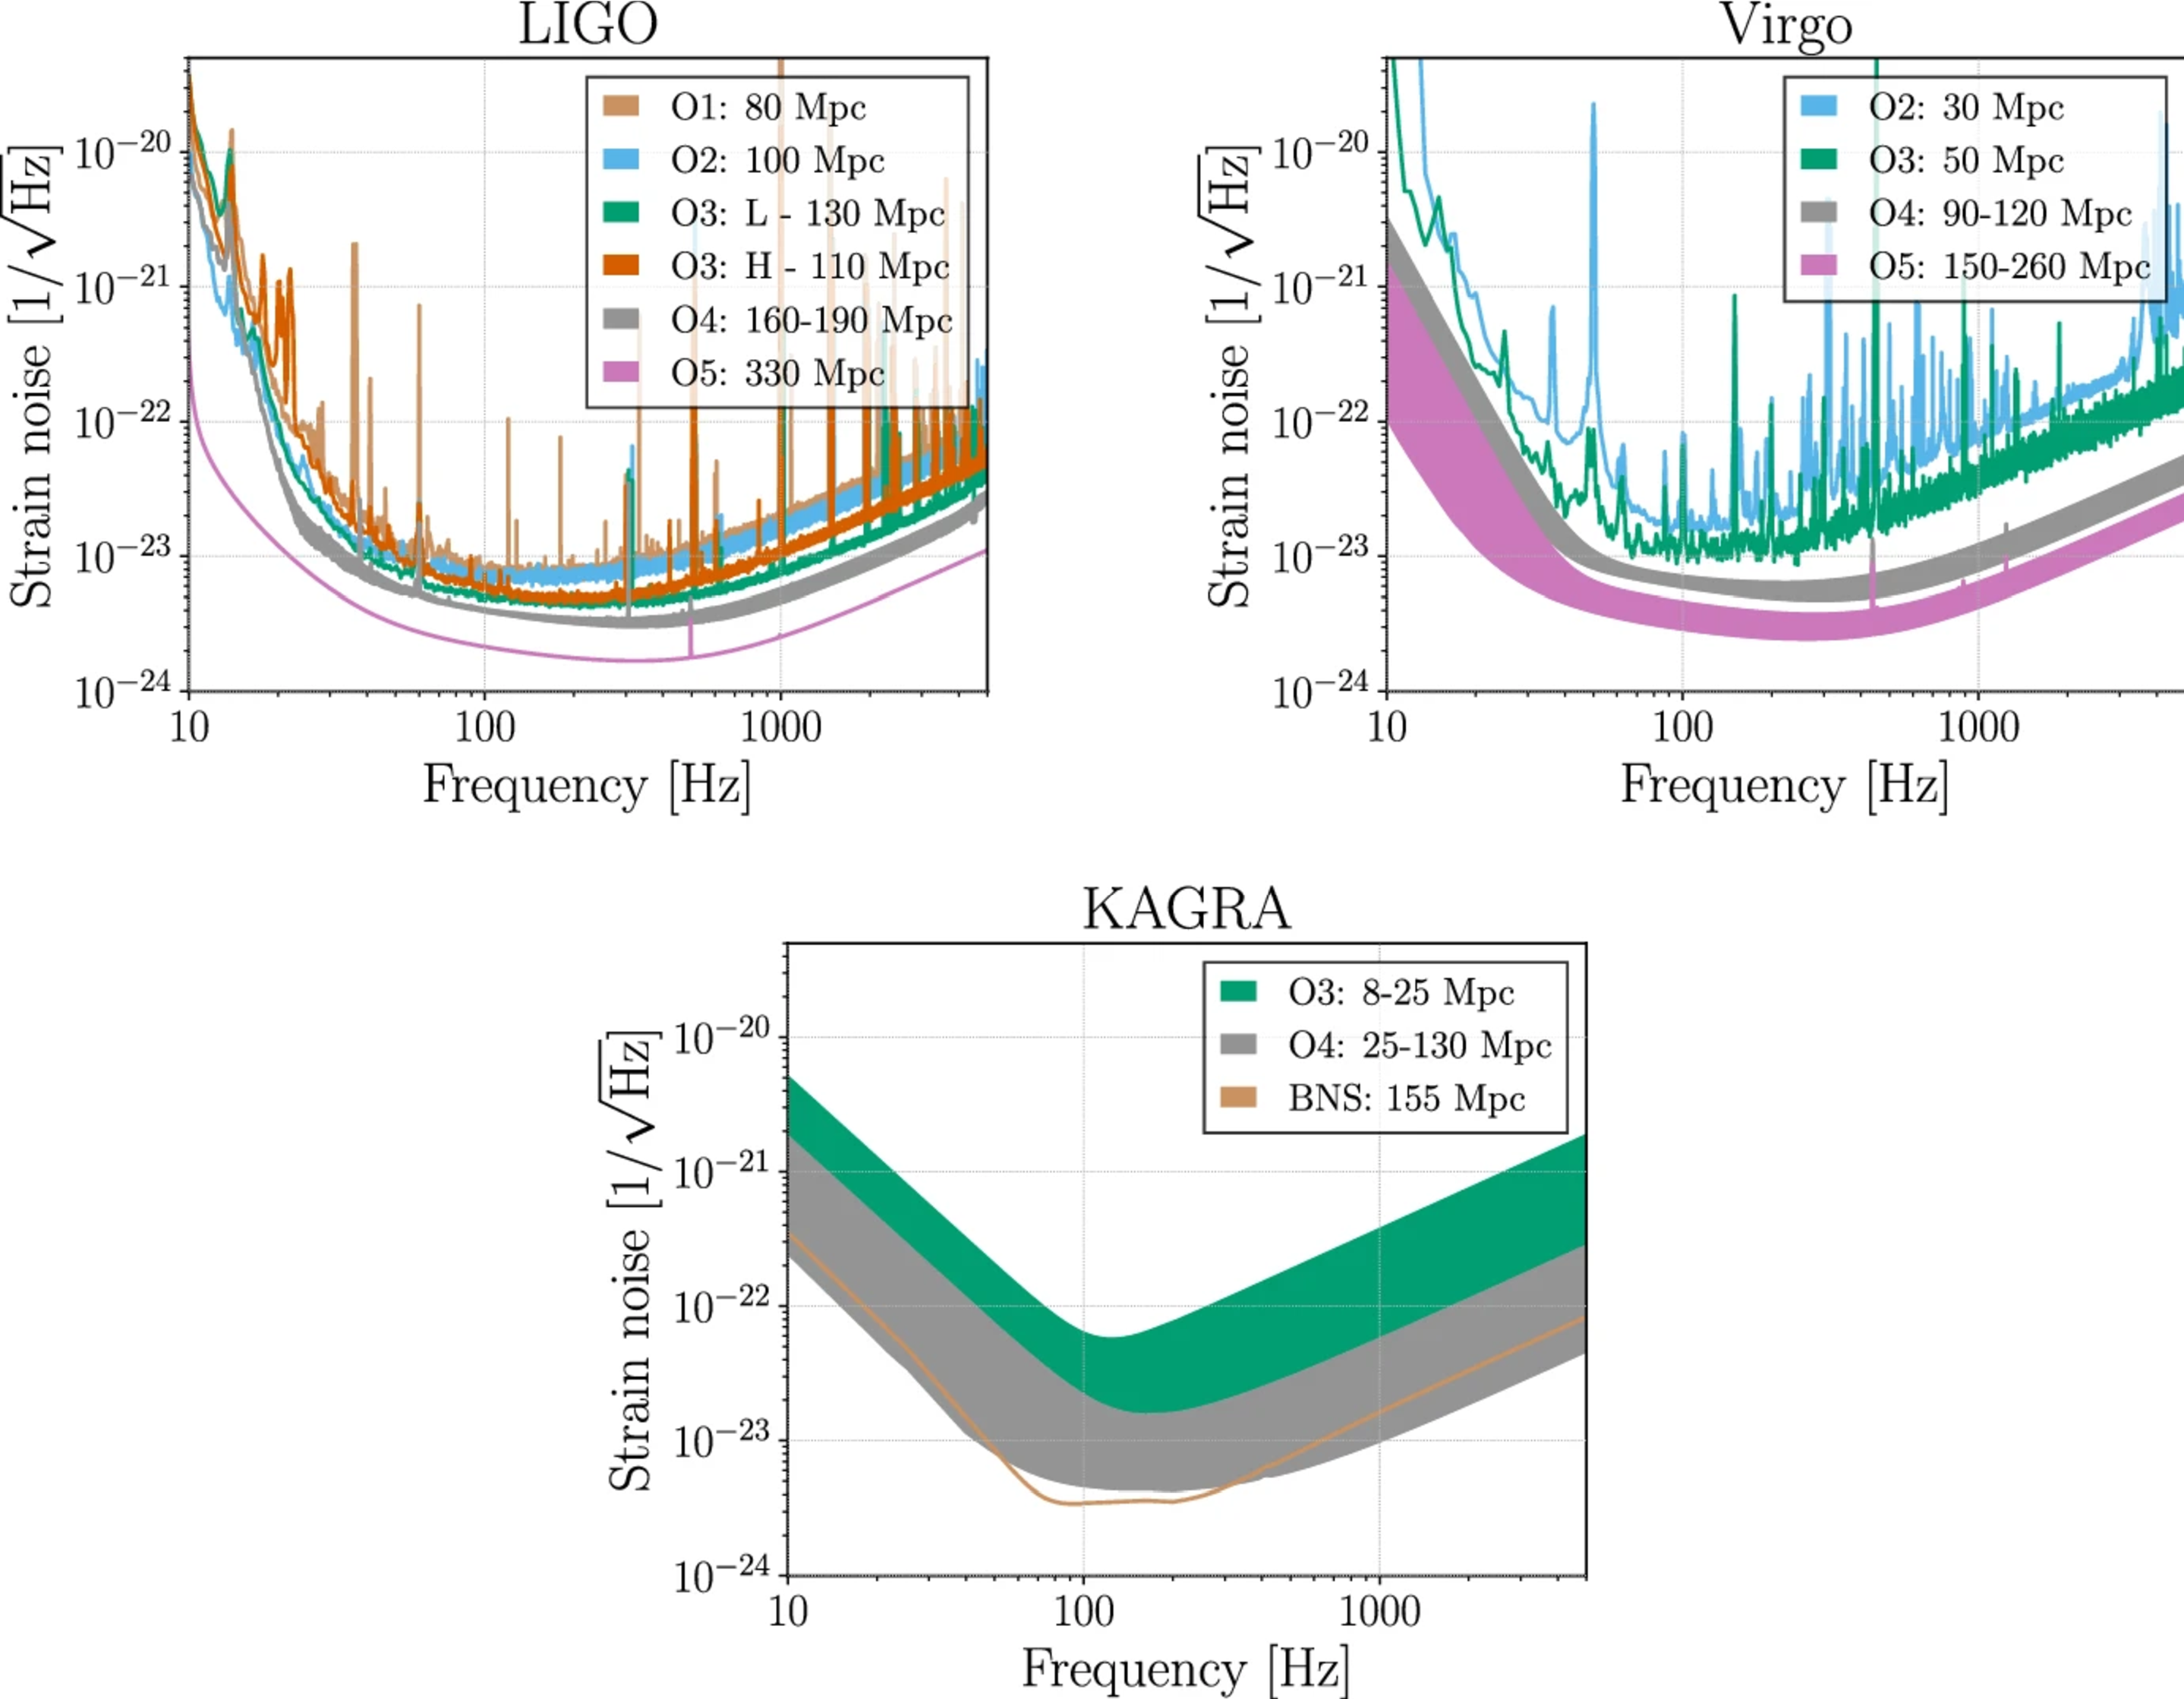
\includegraphics[scale=0.25, angle=0]{figures/Capitolo_3/noiseO4.pdf}
		\setlength{\belowcaptionskip}{-20pt}
		\caption{Prospetti \cite{Abbott_2020a}}
		\label{fig:noiseO4}
	\end{figure}
\end{center}

\lipsum[3]\cite{Abbott_2017a}.

\lipsum[4]\cite{Klimenko_2008}.

\lipsum[6]\cite{Klimenko_2016}.